\documentclass[12pt,reqno]{amsart}
\usepackage{/Users/johnmyers/GoogleDrive/tex/handout,/Users/johnmyers/GoogleDrive/tex/customcommands,polynom}
\usepackage{caption}

\hdr{MAT 240}{\S12.2 Graphs and surfaces; \S12.3 Contour diagrams}

\begin{document}

\textbf{Suggested problems in \S12.2:} 1-13 odd, 19 \medskip

\textbf{Suggested problems in \S12.3:} 5-11 odd, 17

\bigskip
\hrule

\bigskip

\prob Match the graphs with the functions.

\begin{minipage}{0.6\textwidth}
\begin{center}

\includegraphics[scale=1.5]{1.pdf}
\end{center}
\end{minipage}
\begin{minipage}{0.4\textwidth}
\begin{enumerate}
\item $z = 2+x^2+y^2$\bigskip
\item $z = 2-x^2-y^2$\bigskip
\item $z=2(x^2+y^2)$\bigskip
\item $z=2+2x-y$\bigskip
\item $z=2$\bigskip
\end{enumerate}
\end{minipage}

\bigskip
\prob Consider the function $f(x,y) = y^3+xy$. Draw cross sections of $f$ with:

\medskip
\begin{enumerate}
\item $x$ fixed at $x=-1$, $x=0$, and $x=1$\vfill
\item $y$ fixed at $y=-1$, $y=0$, and $y=1$\vfill
\end{enumerate}

\newpage
\prob Plot the surface in $\bbr^3$ defined by the equation $y^2+z^2=1$.

\vfill
\prob The picture below shows a contour diagram of a function $z=f(x,y)$. Use it to estimate the given values of $f(x,y)$.

\bigskip
\begin{center}
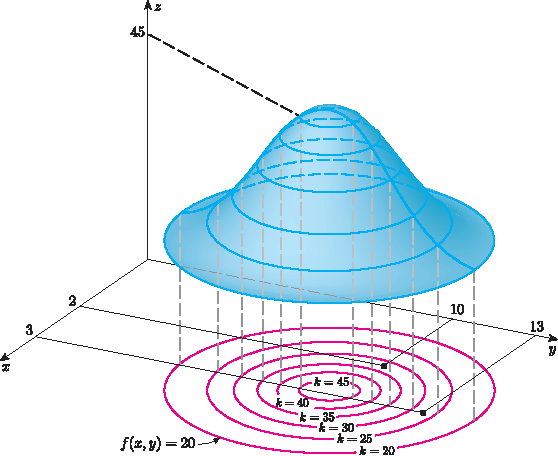
\includegraphics[scale=1.45]{12.pdf}
\end{center}

\bigskip
\begin{henumerate}{2}
\item $f(2,10) \approx$
\item $f(3,13) \approx$
\end{henumerate}

\newpage
\prob Sketch a possible contour diagram for the following surface.

\bigskip

\includegraphics[scale=1.75]{2.pdf}



\vfill
\prob Match the surfaces to the contour diagrams.

\begin{minipage}{0.5\textwidth}
\begin{center}
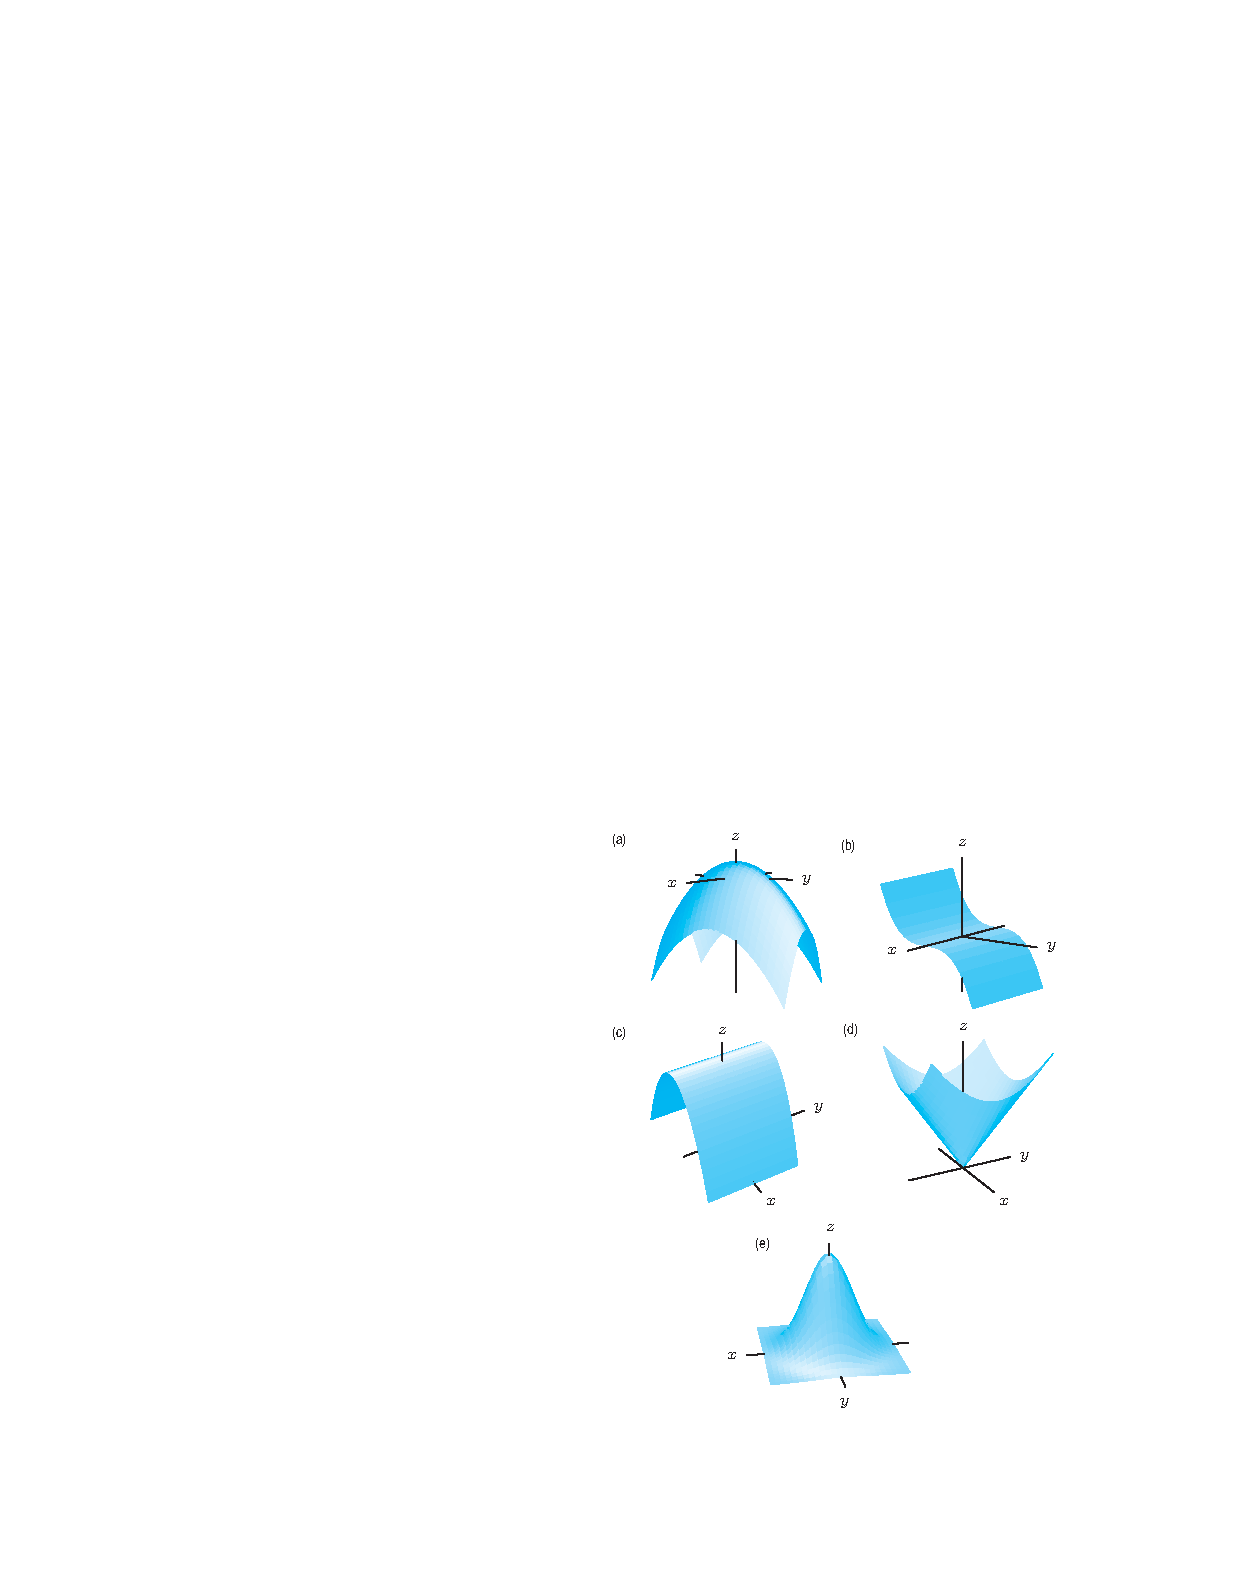
\includegraphics[scale=1]{5.pdf}
\end{center}
\end{minipage}
\begin{minipage}{0.5\textwidth}
\begin{center}
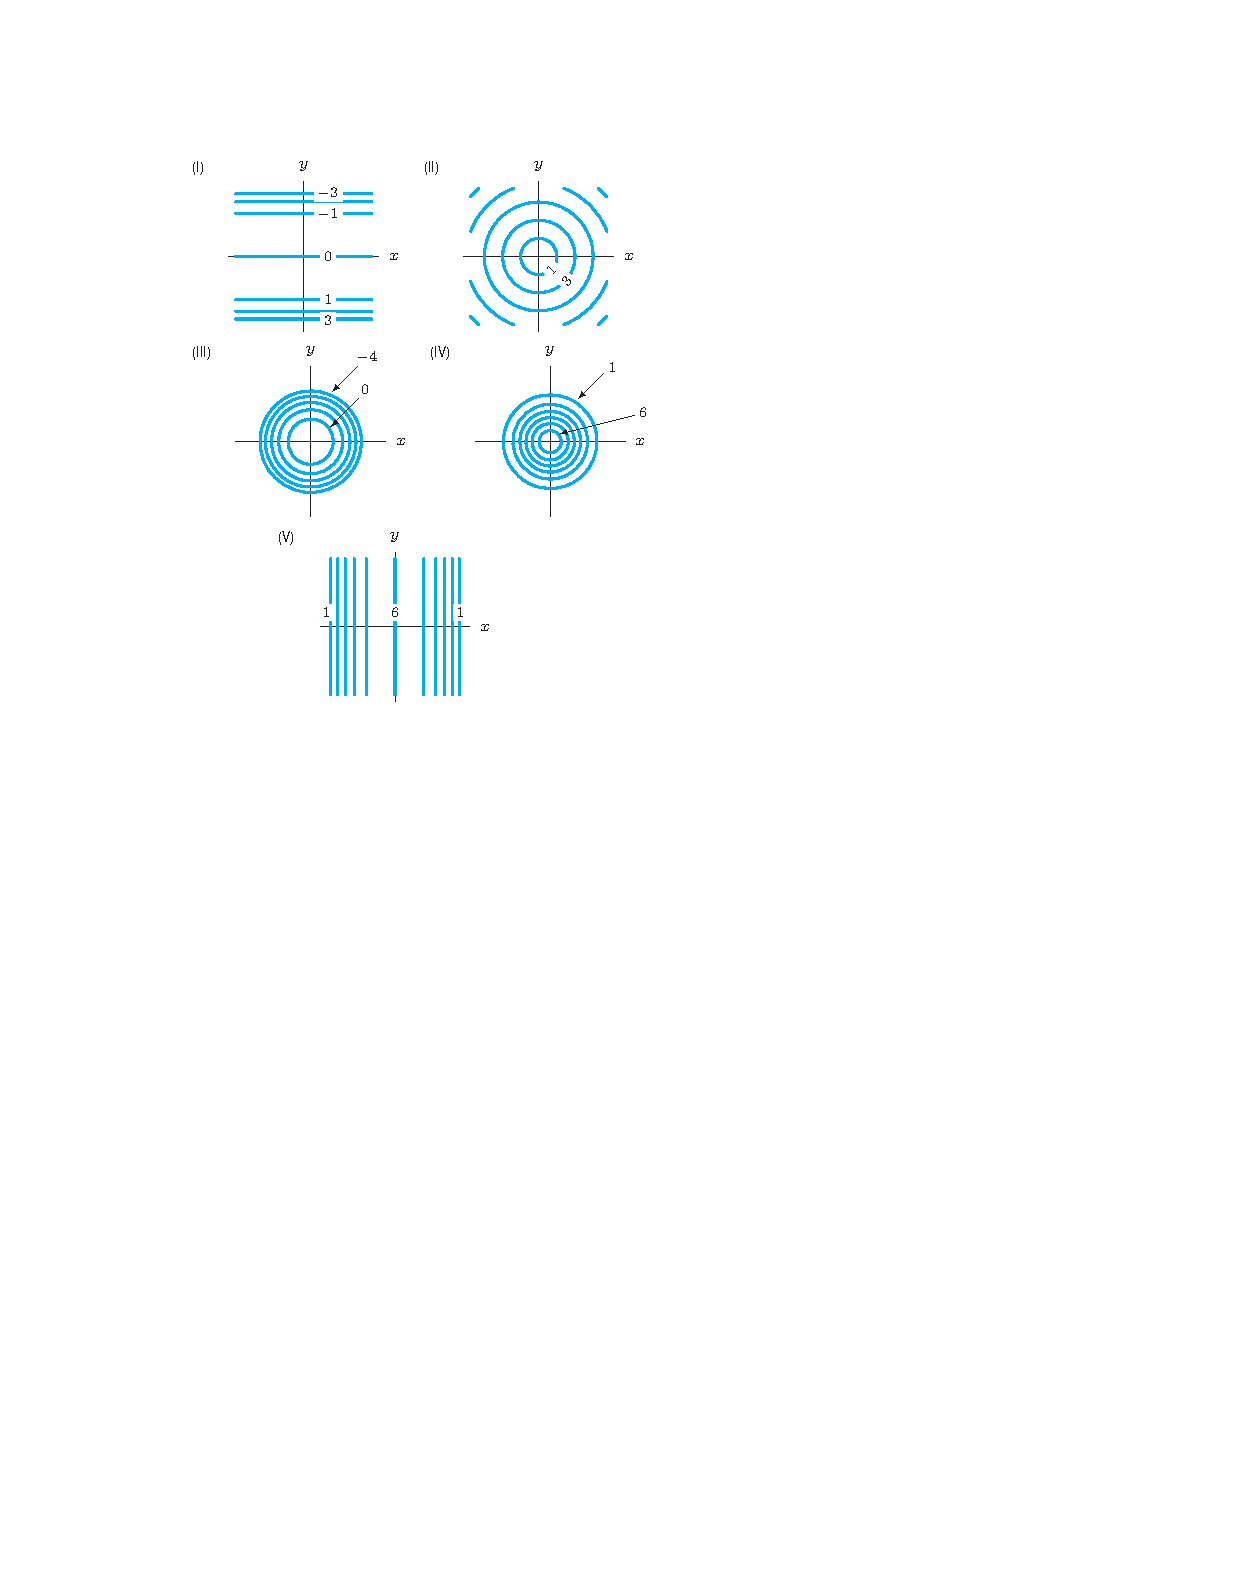
\includegraphics[scale=1]{6.pdf}
\end{center}
\end{minipage}

\vspace{0.5in}
\newpage
\prob Sketch a contour diagram for the graph of $f(x,y) = xy$.


\end{document}